% This is text associated with the open textbook "Open Electromagnetics"
% See immediately below for author, date
% This work is licensed under the Creative Commons Attribution-ShareAlike 4.0 International License. (CC BY-SA 4.0) 
% To view a copy of the license, visit http://creativecommons.org/licenses/by-sa/4.0/

%ORB TITLE Impedance of a Wire
%ORB AUTHOR 0        # S.W. Ellingson, Virginia Tech (ellingson@vt.edu)
%ORB DATE 20191117   # yyyymmdd
%ORB ABSTRACT 

\label{m0159_Impedance_of_a_Wire} % <-- Must match name of this file and module directory name.  Don't mess with this!
\index{impedance!wire|(}

The goal of this section is to determine the impedance -- the ratio of potential to current -- of a wire.
The answer to this question is relatively simple in the DC (``steady current'') case:
The impedance is found to be equal to the resistance of the wire, which is given by
%
\begin{equation}
R = \frac{l}{\sigma A} ~~~~~\mbox{(DC)}
\label{m0159_eRW}    
\end{equation}
where $l$ is the length of the wire and $A$ is the cross-sectional area of the wire.
Also, the impedance of a wire comprised of a perfect conductor
\index{conductor!perfect}
at \emph{any} frequency is simply zero, since there is no mechanism in the wire that can dissipate or store energy in this case.

However, all practical wires are comprised of good -- not perfect -- conductors, 
\index{good conductor}
and of course many practical signals are time-varying, so the two cases above do not address a broad category of practical interest. 
The more general case of non-steady currents in imperfect conductors is complicated by the fact that the current in an imperfect conductor is not uniformly distributed in the wire, but rather is concentrated near the surface and decays exponentially with increasing distance from the surface (this is determined in Section~\ref{m0069_Current_Flow_in_a_Good_Conductor}).

We are now ready to consider the AC case for a wire comprised of a good but imperfect conductor.  
What is the impedance of the wire if the current source is sinusoidally-varying?
Equation~\ref{m0159_eRW} for the DC case was determined by first obtaining expressions for the potential ($V$) and net current ($I$) for a length-$l$ section of wire in terms of the electric field intensity ${\bf E}$ in the wire.  To follow that same approach here, we require an expression for $I$ in terms of ${\bf E}$ that accounts for the non-uniform distribution of current.
This is quite difficult to determine in the case of a cylindrical wire.
However, we may develop an approximate solution by considering a surface which is not cylindrical, but rather planar.  Here we go:

Consider the experiment described in Figure~\ref{m0159_fCFC}. 
%
\begin{figure}[b!]
\begin{center}
\pdftooltip{{  % note double braces
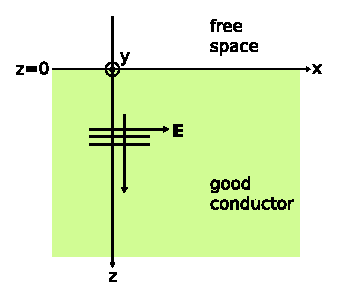
\includegraphics[width=0.8\columnwidth]{modules/m0159_fCFC.eps} 
% https://commons.wikimedia.org ...
}}{An x-y-z coordinate system with x horizontal, z vertical and y out of page. Positive x, negative z region is labeled "free space" and positive z region labeled "good conductor." Electric field capital E moves in positive x direction. Plane wave labeled as moving in the positive z direction.}
\end{center}
\centerline{\scriptsize 
\copyright~\hyperref[m0159_fCFC_Credit]{C.\ Wang} 
\href{https://creativecommons.org/licenses/by-sa/4.0/}{CC BY-SA 4.0} 
} 
\caption{
\label{m0159_fCFC}
Experiment used to determine current density and resistance in the AC case.
}
\end{figure}
% 
Here, a semi-infinite region filled with a homogeneous good conductor meets a semi-infinite region of free space along a planar interface at $z=0$, with increasing $z$ corresponding to increasing depth into the material.
A plane wave propagates in the $+\hat{\bf z}$ direction, beginning from just inside the structure's surface.
The justification for presuming the existence of this wave was presented in Section~\ref{m0069_Current_Flow_in_a_Good_Conductor}.
The electric field intensity is given by
%
\begin{equation}
\widetilde{\bf E} = \hat{\bf x}E_0 e^{-\alpha z} e^{-j\beta z} 
\end{equation}
%
where $E_0$ is an arbitrary complex-valued constant.
The current density is given by Ohm's law of electromagnetics:\footnote{To be clear, this is the ``point form'' of Ohm's law, as opposed to the circuit theory form ($V=IR$).}
\index{Ohm's law}
%
\begin{equation}
\widetilde{\bf J} = \sigma\widetilde{\bf E} = \hat{\bf x}\sigma E_0 e^{-\alpha z} e^{-j\beta z} 
\label{m0159_eJ} 
\end{equation}
% 
Recall that $\alpha = \delta_s^{-1}$ where $\delta_s$ is skin depth (see Section~\ref{m0158_Skin_Depth}). 
\index{skin depth}
Also, for a good conductor, we know that $\beta \approx \alpha$ (Section~\ref{m0157_Good_Conductors}).
Using these relationships, we may rewrite Equation~\ref{m0159_eJ} as follows:
%
\begin{flalign}
\widetilde{\bf J} &\approx \hat{\bf x}\sigma E_0 e^{-z/\delta_s} e^{-jz/\delta_s} \nonumber \\
                  &= \hat{\bf x}\sigma E_0 e^{-(1+j)z/\delta_s}  
\end{flalign}
%
The net current $\widetilde{I}$ is obtained by integrating $\widetilde{\bf J}$ over any cross-section $\mathcal{S}$ through which all the current flows; i.e.,
%
\begin{equation}
\widetilde{I} = \int_{\mathcal{S}} \widetilde{\bf J}\cdot d{\bf s}
\end{equation}
%
Here, the simplest solution is obtained by choosing $\mathcal{S}$ to be a rectangular surface that is perpendicular to the direction of $\widetilde{\bf J}$ at $x=0$.
This is shown in Figure~\ref{m0159_fCFC2}.
%
\begin{figure}
\begin{center}
\pdftooltip{{  % note double braces
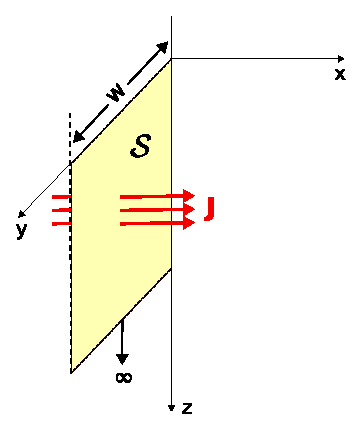
\includegraphics[width=2in]{modules/m0159_fCFC2.eps} 
% https://commons.wikimedia.org ...
}}{An x-y-z coordinate system with x horizontal, z vertical and pointing down, and y coming out of the page. A rectangular surface on the y-z plane is labeled capital S. The width of the rectangle along the y-axis is labeled small w and the length of the rectangle along the z axis is labeled infinity. The plane is moving in the positive x direction with current density labeled capital J.}
\end{center}
\centerline{\scriptsize 
\copyright~\hyperref[m0159_fCFC2_Credit]{Y.\ Zhao} 
\href{https://creativecommons.org/licenses/by-sa/4.0/}{CC BY-SA 4.0} 
} 
\caption{
\label{m0159_fCFC2}
Choice of $\mathcal{S}$ for calculating net current $I$.
}
\end{figure}
%
The dimensions of $\mathcal{S}$ are width $W$ in the $y$ dimension and extending to infinity in the $z$ direction. Then we have 
%
\begin{flalign}
\widetilde{I} &\approx  \int_{y=0}^{W} \int_{z=0}^{\infty} \left( \hat{\bf x}\sigma E_0 e^{-(1+j)z/\delta_s}  \right) \cdot \left( \hat{\bf x}~dy~dz \right) \nonumber \\
  &=  \sigma E_0 W \int_{z=0}^{\infty} e^{-(1+j)z/\delta_s} dz \label{m0159_eI}
\end{flalign}
%
For convenience, let us define the constant $K \triangleq (1+j)/\delta_s$.  Since $K$ is constant with respect to $z$, the remaining integral is straightforward to evaluate:
%
\begin{flalign}
\int_0^{\infty} e^{-Kz}dz &= \left. -\frac{1}{K} e^{-Kz}\right|_0^{\infty} \nonumber \\
                          &= +\frac{1}{K}
\end{flalign}  
%
Incorporating this result into Equation~\ref{m0159_eI}, we obtain:
%
\begin{equation}
\widetilde{I} \approx  \sigma E_0 W \frac{\delta_s}{1+j}
%\label{m0159_eI}
\end{equation}

We calculate $\widetilde{V}$ for a length $l$ of the wire as follows:
%
\begin{equation}
\widetilde{V} = -\int_{x=l}^{0} \widetilde{\bf E}\cdot d{\bf l}
\end{equation}
%
where we have determined that $x=0$ corresponds to the ``$+$'' terminal and $x=l$ corresponds to the ``$-$'' terminal.\footnote{If this is not clear, recall that the electric field vector must point away from positive charge (thus, the $+$ terminal).}
The path of integration can be {\it any} path that begins and ends at the proscribed terminals.  
The simplest path to use is one along the surface, parallel to the $x$ axis.
Along this path, $z=0$ and thus $\widetilde{\bf E}=\hat{\bf x}E_0$.  
For this path:
%
\begin{equation}
\widetilde{V} = -\int_{x=l}^{0} \left(\hat{\bf x}E_0\right)\cdot \left(\hat{\bf x}dx\right) 
  = E_0 l
\label{m0159_eV}
\end{equation}

The impedance $Z$ measured across terminals at $x=0$ and $x=l$ is now determined to be:
%
\begin{equation}
Z \triangleq \frac{\widetilde{V}}{\widetilde{I}} \approx \frac{1+j}{\sigma\delta_s} \cdot \frac{l}{W}
\label{m0159_eCFGC-Z}
\end{equation}
%
The resistance is simply the real part, so we obtain
%
\begin{equation}
R \approx \frac{l}{\sigma(\delta_s W)} ~~~~\mbox{(AC case)}
\label{m0159_eACZ}
\end{equation}
%
The quantity $R$ in this case is referred to specifically as the \emph{ohmic resistance}, since it is due entirely to the limited conductivity of the material as quantified by Ohm's law.\footnote{This is in contrast to other ways that voltage and current can be related; for example, the non-linear $V$-$I$ characteristic of a diode, which is not governed by Ohm's law.}

Note the resemblance to Equation~\ref{m0159_eRW} (the solution for the DC case):  In the AC case, the product $\delta_s W$, having units of area, plays the role of the physical cross-section $S$.  Thus, we see an interesting new interpretation of the skin depth $\delta_s$: 
\index{skin depth}
It is the depth to which a uniform (DC) current would need to flow in order to produce a resistance equal to the observed (AC) resistance.

Equations~\ref{m0159_eCFGC-Z} and \ref{m0159_eACZ} were obtained for a good conductor filling an infinite half-space, having a flat surface. 
How well do these results describe a cylindrical wire?
The answer depends on the radius of the wire, $a$.
For $\delta_s \ll a$, Equations~\ref{m0159_eCFGC-Z} and \ref{m0159_eACZ} are excellent approximations, since $\delta_s \ll a$ implies that most of the current lies in a thin shell close to the surface of the wire.
In this case, the model used to develop the equations is a good approximation for any given radial slice through the wire, and we are justified in replacing $W$ with the circumference $2\pi a$.  Thus, we obtain the following expressions:
%
\begin{equation}
\boxed{
Z \approx \frac{1+j}{\sigma\delta_s} \cdot \frac{l}{2\pi a} ~~~ (\delta_s \ll a)
}
\label{m0159_eZW}
\end{equation}
%
and so
%
\begin{equation}
\boxed{
R \approx \frac{l}{\sigma(\delta_s 2\pi a)} ~~~ (\delta_s \ll a)
}
\label{m0159_eRWAC}
\end{equation}
%
%%%%%%%%%%%%%%%%%%%%%%%%%%%%%%%%%%%%%%%%%%%%%%%
%ORB HIGHLIGHT
\begin{mdframed}[backgroundcolor=yellow!20,nobreak=true] 
The impedance of a wire of length $l$ and radius $a\gg\delta_s$ is given by Equation~\ref{m0159_eZW}.
The resistance of such a wire is given by Equation~\ref{m0159_eRWAC}.
\end{mdframed}
%%%%%%%%%%%%%%%%%%%%%%%%%%%%%%%%%%%%%%%%%%%%%%%

If, on the other hand, $a < \delta_s$ or merely $\sim \delta_s$, then current density is significant throughout the wire, including along the axis of the wire.
In this case, we cannot assume that the current density decays smoothly to zero with increasing distance from the surface, and so the model leading to Equation~\ref{m0159_eZW} is a poor approximation.
The frequency required for validity of Equation~\ref{m0159_eZW} can be determined by noting that $\delta_s \approx 1/\sqrt{\pi f \mu \sigma}$ for a good conductor; therefore, we require
%
\begin{equation}
\frac{1}{\sqrt{\pi f \mu \sigma}} \ll a
\end{equation}
%
for the derived expressions to be valid.  Solving for $f$, we find:
%
\begin{equation}
f \gg \frac{1}{\pi \mu \sigma a^2} 
\label{m0159_efvalid}
\end{equation}
%
For commonly-encountered wires comprised of typical good conductors, this condition applies at frequencies in the MHz regime and above.

These results lead us to one additional interesting finding about the AC resistance of wires.
Since $\delta_s \approx 1/\sqrt{\pi f \mu\sigma}$ for a good conductor, 
Equation~\ref{m0159_eRWAC} may be rewritten in the following form:
%
\begin{equation}
\boxed{
R \approx \frac{1}{2} \sqrt{\frac{\mu f}{\pi \sigma}} \cdot \frac{l}{a}
}
\label{m0159_eACZ2}
\end{equation}
%
We have found that $R$ is approximately proportional to $\sqrt{f}$.  
For example, increasing frequency by a factor of 4 increases resistance by a factor of 2.  
This frequency dependence is evident in all kinds of practical wires and transmission lines.
Summarizing:
%
%%%%%%%%%%%%%%%%%%%%%%%%%%%%%%%%%%%%%%%%%%%%%%%
%ORB HIGHLIGHT
\begin{mdframed}[backgroundcolor=yellow!20,nobreak=true] 
The resistance of a wire comprised of a good but imperfect conductor is proportional to the square root of frequency.
\end{mdframed}
%%%%%%%%%%%%%%%%%%%%%%%%%%%%%%%%%%%%%%%%%%%%%%%

At this point, we have determined that resistance is given approximately by Equation~\ref{m0159_eACZ2} for $\delta_s \ll a$, corresponding to frequencies in the MHz regime and above, and by Equation~\ref{m0159_eRW} for $\delta_s \gg a$, typically corresponding to frequencies in the kHz regime and below.  We have also found that resistance changes slowly with frequency; i.e., in proportion to $\sqrt{f}$. 
Thus, it is often possible to roughly estimate resistance at frequencies between these two frequency regimes by comparing the DC resistance from Equation~\ref{m0159_eRW} to the AC resistance from Equation~\ref{m0159_eACZ2}.  An example follows.

%%%%%%%%%%%%%%%%%%%%%%%%%%%%%%%%%%%%%%%%%%%%%%%
%ORB EXAMPLE
~\\ \begin{example} 
\begin{mdframed}[backgroundcolor=brown!20,linecolor=brown!20]\raggedright
Resistance of the inner conductor of RG-59.
\index{RG-59}
\\~\\
Elsewhere we have considered RG-59 coaxial cable
\index{transmission line!coaxial}
(see the section ``Coaxial Line,'' which may appear in another volume depending on the version of this book).
We noted that it was not possible to determine the AC resistance per unit length $R'$ for RG-59 from purely electrostatic and magnetostatic considerations.
We are now able to consider the resistance per unit length of the inner conductor, which is a solid wire of the type considered in this section.
Let us refer to this quantity as $R'_{ic}$.
Note that 
%
\begin{equation}
R' = R'_{ic} + R'_{oc} 
\end{equation}
%
where $R'_{oc}$ is the resistance per unit length of the outer conductor.
$R'_{oc}$ remains a bit too complicated to address here.
However, $R'_{ic}$ is typically much greater than $R'_{oc}$, so $R' \sim R'_{ic}$.
That is, we get a pretty good idea of $R'$ for RG-59 by considering the inner conductor alone. 

\noindent
The relevant parameters of the inner conductor are
$\mu\approx\mu_0$, 
$\sigma\cong 2.28 \times 10^7$~S/m, and
$a\cong 0.292$~mm.
Using Equation~\ref{m0159_eACZ2}, we find:
%
\begin{flalign}
R'_{ic} &\triangleq \frac{R_{ic}}{l} = \frac{1}{2}\sqrt{\frac{\mu f}{\pi \sigma}} \cdot \frac{1}{a} \nonumber \\
        &\cong \left(227~\mu\Omega\cdot\mbox{m}^{-1}\cdot\mbox{Hz}^{-1/2}\right) \sqrt{f} 
\end{flalign}
%
Using Expression~\ref{m0159_efvalid}, we find this is valid only for $f \gg 130$~kHz.
So, for example, we may be confident that $R'_{ic} \approx 0.82~\Omega$/m at 13~MHz.

At the other extreme ($f \ll 130$~kHz), Equation~\ref{m0159_eRW} (the DC resistance) is a better estimate.
In this low frequency case, we estimate that $R'_{ic} \approx 0.16~\Omega$/m and is approximately constant with frequency.

We now have a complete picture:
As frequency is increased from DC to 13~MHz, we expect that $R'_{ic}$ will increase monotonically from $\approx 0.16~\Omega$/m to $\approx 0.82~\Omega$/m, and will continue to increase in proportion to $\sqrt{f}$ from that value.
%
\end{mdframed}
% note figures will need to go between "\end{mdframed}" and "\end{example}"
\end{example}
%%%%%%%%%%%%%%%%%%%%%%%%%%%%%%%%%%%%%%%%%%%%%%%

Returning to Equation~\ref{m0159_eCFGC-Z}, we see that resistance is not the whole story here.  
The impedance $Z=R+jX$ also has a reactive component $X$ equal to the resistance $R$; i.e.,
%
\begin{equation}
X \approx R \approx \frac{l}{\sigma(\delta_s 2\pi a)}
\end{equation}
%
This is unique to good conductors at AC; that is, we see no such reactance at DC.
Because this reactance is positive, it is often referred to as an inductance.
\index{inductance}
However, this is misleading since inductance refers to the ability of a structure to store energy in a magnetic field, and energy storage is decidedly \emph{not} what is happening here.
The similarity to inductance is simply that this reactance is positive, as is the reactance associated with inductance.
As long as we keep this in mind, it is reasonable to model the reactance of the wire as an \emph{equivalent} inductance:
\index{inductance!equivalent}
%
\begin{equation}
L_{eq} \approx \frac{1}{2\pi f} \cdot \frac{l}{\sigma(\delta_s 2\pi a)} 
\end{equation}
%
Now substituting an expression for skin depth:
%
\begin{flalign}
L_{eq} &\approx \frac{1}{2\pi f} \cdot \sqrt{\frac{\pi f \mu}{\sigma}} \cdot \frac{l}{2\pi a} \nonumber \\
       &= \frac{1}{4\pi^{3/2}} \sqrt{\frac{\mu}{\sigma f}} \cdot \frac{l}{a}
\label{m0159_eLeq2}
\end{flalign}
%
for a wire having a circular cross-section with $\delta_s\ll a$.
The utility of this description is that it facilitates the modeling of wire reactance as an inductance in an equivalent circuit.
Summarizing: 
%
%%%%%%%%%%%%%%%%%%%%%%%%%%%%%%%%%%%%%%%%%%%%%%%
%ORB HIGHLIGHT
\begin{mdframed}[backgroundcolor=yellow!20,nobreak=true] 
A practical wire may be modeled using an equivalent circuit consisting of an ideal resistor (Equation~\ref{m0159_eACZ2}) in series with an ideal inductor (Equation~\ref{m0159_eLeq2}).  Whereas resistance increases with the square root of frequency, inductance \emph{decreases} with the square root of frequency.
\end{mdframed}
%%%%%%%%%%%%%%%%%%%%%%%%%%%%%%%%%%%%%%%%%%%%%%%

If the positive reactance of a wire is not due to physical inductance, then to what physical mechanism shall we attribute this effect?
A wire has reactance because there is a phase shift between potential and current.
This is apparent by comparing Equation~\ref{m0159_eI} to Equation~\ref{m0159_eV}.  
This is the same phase shift that was found to exist between the electric and magnetic fields propagating in a good conductor, as explained in Section~\ref{m0157_Good_Conductors}.

%%%%%%%%%%%%%%%%%%%%%%%%%%%%%%%%%%%%%%%%%%%%%%%
%ORB EXAMPLE
~\\ \begin{example} 
\begin{mdframed}[backgroundcolor=brown!20,linecolor=brown!20]\raggedright
Equivalent inductance of the inner conductor of RG-59.
\index{RG-59}
\\~\\
Elsewhere in the book we worked out that the inductance per unit length $L'$ of RG-59 
coaxial cable 
\index{transmission line!coaxial}
was about $370$~nH/m.
We calculated this from magnetostatic considerations, so the reactance associated with skin effect 
\index{skin effect}
is not included in this estimate.
Let's see how $L'$ is affected by skin effect for the inner conductor.
Using Equation~\ref{m0159_eLeq2} with 
$\mu=\mu_0$, 
$\sigma\cong 2.28 \times 10^7$~S/m, and
$a\cong 0.292$~mm, we find
%
\begin{equation}
L_{eq} \approx \left( 3.61 \times 10^{-5}~\mbox{H$\cdot$m$^{-1}\cdot$Hz$^{1/2}$} \right) \frac{l}{\sqrt{f}} 
\end{equation}
%
Per unit length:
%
\begin{equation}
L_{eq}' \triangleq \frac{L_{eq}}{l} \approx \frac{3.61 \times 10^{-5}~\mbox{H$\cdot$Hz$^{1/2}$}}{\sqrt{f}} 
\end{equation}
%
This equals the magnetostatic inductance per unit length ($\approx 370$~nH/m) at $f \approx 9.52$~kHz, and decreases with increasing frequency.

Summarizing:  The equivalent inductance associated with skin effect is as important as the magnetostatic inductance in the kHz regime, and becomes gradually less important with increasing frequency.
\end{mdframed}
% note figures will need to go between "\end{mdframed}" and "\end{example}"
\end{example}
%%%%%%%%%%%%%%%%%%%%%%%%%%%%%%%%%%%%%%%%%%%%%%%

Recall that the phase velocity in a low-loss transmission line is approximately $1/\sqrt{L'C'}$.  
This means that skin effect causes the phase velocity in such lines to decrease with decreasing frequency.
In other words:
%
%%%%%%%%%%%%%%%%%%%%%%%%%%%%%%%%%%%%%%%%%%%%%%%
%ORB HIGHLIGHT
\begin{mdframed}[backgroundcolor=yellow!20,nobreak=true] 
Skin effect in the conductors comprising common transmission lines leads to a form of dispersion in which higher frequencies travel faster than lower frequencies.
\end{mdframed}
%%%%%%%%%%%%%%%%%%%%%%%%%%%%%%%%%%%%%%%%%%%%%%%
%
This phenomenon is known as \emph{chromatic dispersion}, or simply ``dispersion,'' 
\index{dispersion}
and leads to significant distortion for signals having large bandwidths.

%%%%%%%%%%%%%%%%%%%%%

{\bf Additional Reading:}
\begin{itemize}
\item ``\href{https://en.wikipedia.org/wiki/Skin_effect}{Skin effect}'' on Wikipedia.
\end{itemize}

\index{impedance!wire|)}


